
\setcounter{chapter}{4}
%----------------------------------------------------------------------------
\chapter*{4. Tétel}
%----------------------------------------------------------------------------

\textbf{Témakörök:} A lineáris programozás dualitástétele (két alakban). A lineáris programozás alapfeladatának bonyolultsága (biz. nélkül).

\noindent\hrulefill

\section*{LP feladatok alakjai}
Drakula Művek példája $c=(12,12)$ célfüggvény mellett:

\begin{figure}[h!]
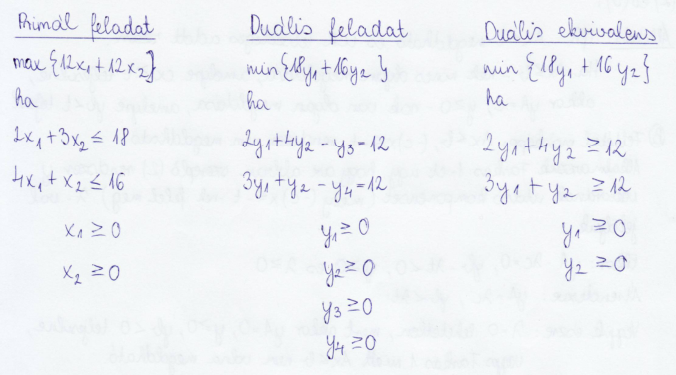
\includegraphics[width=14cm]{lp_alakok}
\centering
\end{figure}

\textbf{Megjegyzés:} $y_{3}$ és $y_{4}$ elhagyása a rendszerből nem befolyásolja a megoldhatóságot, sem a célfüggvényértéket. Az ekvivalens alak már könnyen ábrázolható grafikusan a síkon. Ha a primál feladatban elő van írva a változók nemnegatív értékűsége, akkor a duális esetében sem szabad erről megfeledkezni!

\section*{Dualitás tétel}

\begin{theo} 
Ha a $max \lbrace c x: Ax\leq b\rbrace$ primál program megoldható és felülről korlátos:
\begin{enumerate}
\item	a $min \lbrace yb: yA=c,y\geq 0\rbrace$ duális program is megoldható és alulról korlátos,
\item	a primál programnak létezik maximuma és a duális programnak létezik minimuma,
\item	továbbá ezek megegyeznek: $max\lbrace cx: Ax\leq b\rbrace = min\lbrace yb: yA=c,y\geq 0\rbrace$
\end{enumerate}
\end{theo}
\textbf{Megjegyzés:} $(2)$-re szükség van, mert egy számhalmaz felülről korlátosságából általában nem következik, hogy létezik maximuma.

\section*{Ekvivalens alak}
\begin{theo}
Ha a $max\lbrace cx:AX\leq b,x\geq 0\rbrace$ primál program megoldható és felülről korlátos:
\begin{enumerate}
\item a $min \lbrace yb:yA\geq c, y \geq 0\rbrace$ duális program is megoldható és alulról korlátos,
\item	a primál programnak létezik maximuma és a duális programnak létezik minimuma,
\item	továbbá ezek megegyeznek: $max\lbrace cx:AX\leq b,x\geq 0\rbrace = min \lbrace yb:yA\geq c, y \geq 0\rbrace$
\end{enumerate}
\end{theo}

\section*{Bonyolultság}
\subsection*{LP feladat, eldöntési problémaként megfogalmazva}
Van-e az $Ax\leq b$ feltételt kielégítő $x$ vektorok között olyan, amelyre $cx\geq t$?
\begin{itemize}
	\item NP-beli: tanú egy ilyen $x$
	\item co-NP-beli: ha $cx<t$, akkor a duális megoldása ($y$) tanú erre
	\item (a tanúk polinomiális méretűek)
\end{itemize}

\subsection*{Módszerek}
\begin{itemize}
\item Szimplex módszer (1947, Dantzig): nem polinomiális, de a gyakorlati alkalmazások során gyors
\item Ellipszoid módszer (1979, Hacsijan): polinomiális, de a gyakorlati alkalmazások során lassú
\item Belső pontos módszerek (1984, Karmarkar): polinomiális, a gyakorlati alkalmazások során eredményes, de nem elterjedt
\end{itemize}
